\chapter{Introducción}






\section{Motivación}

Este trabajo es importante por que 



\section{Marco Teórico}



\subsection{Análisis de sentimiento y emociones en el texto}

Las seres humanos atravesamos la experiencia de la vida a través de nuestra cognición, es decir, el conjunto de procesos mentales que culminan en la representación interna del mundo que nos rodea. Una parte fundamental de esta, son las emociones. En un esfuerzo por intentar identificarlas de una manera generalizada, Ekman \cite{ekman1993facial}  realiza un estudio de la respuesta fisiológica en general y de las  expresiones faciales en particular, del ser humano en diferentes culturas ante distintas circunstancias. Esto lo lleva a concluir que existen grandes grupos en donde las distintas expresiones faciales pueden ser agrupadas ya que estas reflejan el estado emocional interno de los individuos. A estos grupos los denomino emociones básicas y son los siguientes: Alegría, enojo, sorpresa, asco, miedo y tristeza. Este modelo de emociones básicas es comúnmente usado para los estudios relacionados con las emociones. 

Debido la relevancia que presentan las emociones en la manera en como procesamos la informacion, en el libro \cite{picard2000affective} Picard pone de manifiesto que la búsqueda de una inteligencia artificial capaz de interactuar eficazmente con los seres humanos, debe traer consigo la capacidad de reconocer, entender, tener y expresar emociones. Es así como bautiza el capo de estudio que busca dicha interacción como computación afectiva, y expone los avances hechos hasta la fecha en el mismo.

Dado que el lenguaje en general es el medio principal mediante el cual los seres humanos transferimos informacion de manera general, y mediante las computadoras en particular, los esfuerzos orientados hacia esta computación afectiva tienen un componente fundamental en el procesamiento del lenguaje para dicho propósito, por lo que se genera la necesidad de entender la relación que existe entre lenguaje y emoción antes de poder automatizar este proceso. Dentro de este marco, \cite{ortony1987referential} se habla de como a pesar de que las emociones son procesos mentales internos que no residen en el lenguaje, este es el medio no fenomenológico mas conveniente a través del cual podemos acceder a ellas. Elabora entonces una serie condiciones que deben estar presentes en los términos para poder referirse de una manera acertada a los estados emocionales, y las aplica sobre términos presentes en la literatura con respecto a las emociones, construyendo así un léxico emocional. De manera análoga, \cite{hatzivassiloglou1997predicting} construye a partir de un corpus extenso de adjetivos que vienen en parejas usando distintos conectores, y un etiquetado manual de algunos de ellos, un algoritmo para determinar lo que los autores denominan la orientación semántica de los mismos, esto es determinar si determinado adjetivo tiene una connotación negativa o positiva de la característica que describe. Este método permite la creación automática de un corpus extenso de adjetivos cuyo sentimiento se encuentra identificado.

Mas allá de la relación individual que existe entre palabras y estados emocionales,  \cite{wiebe1994tracking} a través del análisis de un tipo particular de texto, la ficción, expone que la narración puede ocurrir desde un punto de vista objetivo, es decir, una descripción de hechos comprobables, y también desde un punto de vista subjetivo, es decir, poniendo de manifiesto los hechos atravesados por los estados mentales internos del narrador, y que la distinción entre un tipo de narración y otra no esta siempre clara, por lo que propone un algoritmo capaz de hacer esta distinción de manera automática. Esto es retomado por \cite{yu2003towards} en donde se busca hacer esta distinción a nivel de documentos, por ejemplo diferenciar editoriales  de noticias, así como a nivel de frases mediante el uso modelos de aprendizaje supervisado para estas tareas en particular.

De una manera general, los estados emocionales internos de las personas que ocurren como respuesta a los eventos externos pueden ser agrupados según su polaridad, es decir, catalogar el sentimiento como positivo o negativo. Es así como  \cite{pang2002thumbs}  establece la importancia de desarrollar, ante textos que reflejen opiniones subjetivas, sistemas capaces de identificar si dicha opinión es negativa o positiva. Para este propósito, se emplea el dominio de las reviews online de películas, que facilitan la tarea al contar con una valoración negativa o positiva por parte del usuario, construyendo algoritmos de aprendizaje supervisado que utiliza como features principalmente unigramas, que es un elemento inidivudual del texto y como variable objetivo el sentimiento la valoración expresada. Por otro lado,  \cite{turney2002thumbs} pretende establecer a través de aprendizaje no supervisado, si determinada review sobre diversos temas online, presenta un sentimiento negativo o positivo. Para ello, emplea el concepto de orientación semántica presente en \cite{hatzivassiloglou1997predicting} para determinar si una frase tiene orientación negativa o positiva para luego determinar si la review en su conjunto es positiva o negativa. En general, la determinación de la orientación negativa o positiva dentro del texto, es conocida como análisis de sentimiento

Así como en el análisis de sentimiento, contar con un corpus de términos que cuenten con una clasificación previa de su orientación es clave para poder llevar a cabo automáticamente la tarea, para los estados emocionales  es igualmente importante, por lo que \cite{strapparava2004wordnet} realiza una anotación manual de estados emocionales basados en las categorías de \cite{ortony1987referential} sobre algunos términos encontrados en WordNet \cite{miller1995wordnet}, que es una base de datos de términos en ingles agrupados por grupos de sinónimos y con relación semántica entre grupos. A partir de ahí se establece la categoría emocional de nuevos términos gracias a los sinónimos y las relaciones semánticas, construyendo así una base de datos de estados emocionales llamada WordNet-Affect. Dentro de esta misma linea, \cite{wiebe2005annotating}  elabora una anotación manual de las estados emocionales presentes en las oraciones de un gran volumen de noticias, en donde se tiene en cuenta el contexto. 

Mas allá de la relación entre términos particulares y estados emocionales, \cite{alm2005emotions} utilizan los cuentos infantiles para desarrollar un modelo de aprendizaje supervisado capaz de detectar emociones en las frases del texto. Para ello se elabora una anotación manual de las frases que constituyen el set de datos y luego, se generan un set de features para estas que pasaran a entrenar un clasificador lineal.



\subsection{Sentimientos y emociones en redes sociales}

Con el paso del tiempo, Internet se han convertido en un lugar de intercambio de informacion prevalente entre sus usuarios y dicha informacion se presenta, entre otras formas, en el texto, por ello, es una fuente de generación masiva del mismo que puede facilitar su estudio. En ese sentido, \cite{pang2008opinion} se hace manifiesto la importancia que ha venido ganando el campo del análisis de sentimiento del texto en Internet, tanto para usuarios individuales como para la industria de la publicidad, el mercado financiero y la academia, por lo que se hace un recuento de las distintas técnicas y aplicaciones que son consideradas relevantes por los autores hasta la fecha.

Un espacio particular en donde los usuarios individuales pueden generar grandes volúmenes de informacion sobre distintos contenidos, y por consiguiente, una fuente rica de datos para el análisis de sentimiento son los blogs. Por esta razón, \cite{aman2007identifying} utiliza texto proveniente de ellos para realizar detección de emociones presentes en las oraciones de los mismos. Para este propósito recurren primero a una anotación manual de las mismas y luego a la construcción de features para entrenar distintos modelos supervisados. 

Twitter, un sitio de blogs en particular cuyo formato es el microblogging, es decir, publicaciones pequeñas a las que denomina tweets, ha cobrado una gran relevancia en el estudio del texto debido a su gran popularidad entre los usuarios de Internet de todo tipo, desde marcas, usuarios individuales y políticos, para abarcar cualquier tema. En ese contexto,  \cite{pak2010twitter} extrae tweets de diferentes usuarios sobre distintos temas para realizar un análisis de sentimientos sobre estos. Para ello se procede  a la identificación de tweets que contengan emoticones felices y tristes, los cuales etiqueta como reflejando un sentimiento positivo o negativo respectivamente, así como tweets provenientes de cuentas de medios de noticias los cuales etiqueta como neutrales. luego se procede a la construcción de features usando n-gramas, que son elementos que contienen la combinación de n palabras del texto, a partir de las palabras presentes en el tweets  con estos se entrenaron varios clasificadores. 

Un elemento característico de twitter, son los hashtags que consisten en palabras precedidas del signo numeral (\#) y sirven para denotar una temática en particular relacionada con el tweet, por ejemplo "\#emociones". Gracias a esta potencial para categorizar de los hashtags,\cite{davidov2010enhanced} parte del supuesto de que estos y los emoticones contienen información relevante el cuanto al sentimiento del tweet, por lo que partiendo de una base de datos de 475 millones de tweets publicados entre mayo del 2009 y enero del 2010, se hace una selección de 50 hashtags que tengan una asociación fuerte a sentimientos y se entrena un modelo supervisado a partir de los tweets que contengan estos hashtags, representándolos a través de vectores de features . El modelo es posteriormente empleado para clasificar otros tweets y jueces humanos verifican su eficacia. Una idea similar emplea \cite{wang2012harnessing}, en donde este concepto sirvió ademas para la extracción de datos pues  se utilizan hashtags que contengan términos claves provenientes de las 5 emociones básicas de propuestas por \cite{ekman1993facial} para realizar el llamado de la API (application programming interface) de Twitter, es decir, solicitando del sitio que se extraigan solo los tweets que contengan estos hashtags. Esta manera de utilizar los hashtags como un tipo de clasificación, es conocida como supervisado distante.

Si bien el método de supervisado distante puede servir como una estimación de la relación entre el texto del tweet y su contenido emocional, es un método en el que no se puede afirmar con certitud dicha relación. Por ello, \cite{roberts2012empatweet} identifica la necesidad de contar con un corpus etiquetado que sirva de base para la tarea de identificación de emociones en twitter. Para ello, se seleccionan  14 temas que para los autores tienen un fuerte contenido emocional y las palabras clave asociados a estos para ser usados como hashtags en las extracción. A partir de ahí, manualmente se etiquetaron los tweets con su respectiva emoción. Esto sirvió de base para entrenar un modelo de aprendizaje supervisado y así verificar el poder predictivo de los modelos partiendo de datos etiquetados.

La identificación del sentimiento presente en Twitter puede servir como fuente de aproximación a la realidad social en la que los usuarios se desenvuelven debido a la naturaleza inmediata, relevante para los usuarios y descentralizada propia del flujo de informacion de esta red social. Por esto,
 \cite{o2010tweets} se plantea la pregunta si existe una correlación entre el sentimiento encontrado en twitter y las encuestas de opinión. Para ello, se toma una muestra del de mil millones de tweets entre 2008 y 2009 y se toman aquellos tweets que contengan palabras claves asociadas a los temas que se están investigando. EL sentimiento de estos tweets se determina a partir de la proporción de palabras con asociación negativa o positiva presentes en el tema que se esta analizando en un día en particular. Los resultados dan una correlación alta entre el sentimiento encontrado a través del texto y las encuestas. Esta relación entre la realidad social y el sentimiento presente en los tweets es también abordada por \cite{bollen2011modeling}, donde se procede a realizar una medida del estado emocional de una muestra de tweets entre agosto y diciembre del 2008, en donde el mismo se mide a través de la similaridad presente entre las palabras de los tweets y ciertos términos claves asociados a estados emocionales. Esto permite encontrar que determinados eventos relevantes generan un impacto emocional significativo y durante un periodo de tiempo en los usuarios.

Al ser el escenario político un caso particular de los fenómenos sociales cuyo impacto se traduce en el estado emocional de las personas, el sentimiento presente en tweets de contenido político puede dar un indicio de la percepción publica de dicho escenario. Con esto en mente, \cite{tumasjan2010predicting} se plante el uso de twitter como plataforma de medición de la percepción publica respeto a la política durante las elecciones parlamentarias en Alemania en el 2009. Una de sus preguntas de investigación estuvo relacionada con los sentimientos que se reflejan en los tweets que mencionan a los políticos que hacen parte de las campañas y para esto, se empleo sobre el texto proveniente de twitter, un software capaz de identificar palabras claves asociadas a estados emocionales y cognitivos en el texto. El resultado fue un perfil emocional para cada político que en lineas generales, parece estar de acuerdo con su discurso político. Esta relación entre política y sentimiento presente en twitter, fue también  estudiada por  \cite{ceron2016sentiment} en donde realizó un análisis de sentimientos sobre tweets relacionados con las elecciones presidenciales en Colombia en el 2014 y se compararon los resultados de este con las encuestas de opinión. Para ello, inicialmente obtiene tweets que tengan  palabras claves y hashtags relacionados con las elecciones, luego hace un filtrado de spam y finalmente entrena un modelo supervisado con los features que genera para los tweets restantes. Los resultados no son consistentes por lo que se plantea en futuros trabajos  una caracterización demográfica.

\subsection{Redes neuronales para el análisis de texto}

Las técnicas tradicionales de análisis de sentimiento y emociones están principalmente basadas en la relación que existe entre los términos que constituyen el texto y determinado estado emocional. Este tipo de análisis, si bien ha sido de gran utilidad, no dispone de la capacidad de tener en cuenta el contexto, es decir la relación que existe entre las palabras que constituyen el texto y el orden en que estas se presentan. Debido a esto, recientemente el campo de ido migrando hacia el uso del algoritmos capaces de captar esta relación contextual, específicamente las redes neuronales. Bajo perspectiva, \cite{acheampong2021transformer} hace un recuento del estado del arte de la detección de emociones en el texto. Es aquí donde se pone en evidencia la conveniencia de usar RNN (redes neuronales recurrentes) debido a la naturaleza secuencial de su arquitectura. 

Las RNN (redes neuronales recurrentes) son un tipo de arquitectura de red neuronal cuyo uso es especial para datos secuenciales, tales como las tareas de NLP. En estas, para un ejemplo nuevo, es posible utilizar el resultado del procesamiento de un dato anterior, para el del siguiente dato (como en una secuencia de caracteres por ejemplo), es decir la misma topología de pesos recibirá para cada ejemplo nuevo, el resultado anterior ademas de la nueva entrada. En la imagen \ref{figure:RNN} \cite{enwiki:1109264340} se evidencia un esquema de esta arquitectura.


\begin{figure}[h]
	\caption{Red neuronal recurrente}
	\centering
	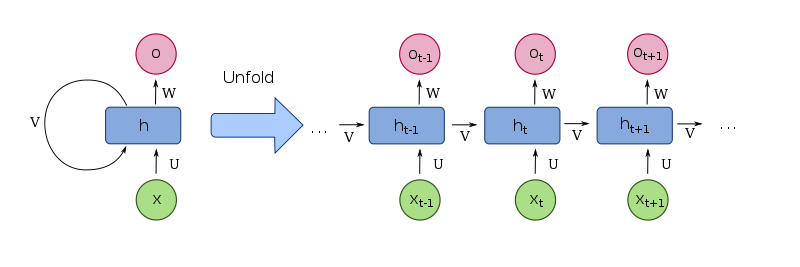
\includegraphics[scale=0.55]{Images & Logos/Recurrent_neural_network_unfold.svg.png} 
	\label{figure:RNN}
\end{figure}

 Sin embargo, debido a su arquitectura, la optimizacion de los pesos que constituyen la topología de las RNN, se vuelve compleja pues para el calculo del gradiente del error, pues se deberá pasar tantas veces por los pesos de la red como pasos en el tiempo haya (como numero de caracteres en una palabra) haciendo que en secuencias particularmente largas, este calculo crezca o disminuya en demasía. Para enfrentar este problema , \cite{hochreiter1997long} y \cite{chung2014empirical} plantean nuevas arquitecturas de RNN conocidas como LSTM (Long-Short term memoryzz) y GRU (Gated Recurrent Unit) respectivamente, en donde a través de nuevas unidades que permiten la activación/cancelación de las señales que constituyen la red, se puede realizar la optimizacion de manera directa sin pasar por los pesos.

 Luego se describe como el uso de Transformers permitió paralelizár el procesamiento, así como la capacidad de tener información contextual para intervalos secuenciales mas amplias. Dentro del uso de Transformers se resalta el uso de modelos pre entrenados que puedan ser utilizados para tareas especificas a través de un entrenamiento final. Acá se resalta BERT como el modelo mas popular para la tarea de detección de emociones recientemente.







Si bien las RNN permiten preservar de alguna manera la relación contextual del texto, al tener una estructura secuencial, se impide la paralelizacion de su computo, pues se necesita las salidas de ejemplos anteriores para llevar a cabo el siguiente paso en el tiempo. Ademas, debido a este mismo funcionamiento secuencial, si existe un gran numero de pasos en el tiempo, es poco probable que la red tenga en cuenta información presente al inicio. Para solucionar estos inconvenientes, \cite{vaswani2017attention} desarrollan los Transformers, que son un tipo de arquitectura en la que múltiples datos de entrada son ingresados a la red de manera simultanea, como todas las palabras en una frase por ejemplo, mediante la representación de dichas palabras en la forma de un vector (Embedding) y a través de una arquitectura que definen como atención, se realiza una transformación de los datos de manera que la representación de cada dato, en este caso cada palabra, tenga en cuenta que tan importante es la misma para todas las demás palabras de la oración. Esta transformación, aplicada tanto en los datos de entrada como en los de salida, es luego usada para entrenar los pesos de la red. De esta manera la red es capaz de procesar datos en simultaneo así como tener en cuenta toda la información disponible. Un esquema de esta arquitectura se puede apreciar en la imagen \ref{figure:transformers} \cite{vaswani2017attention}.

\begin{figure}[h]
	\caption{Arquitectura de los Transformers}
	\centering
	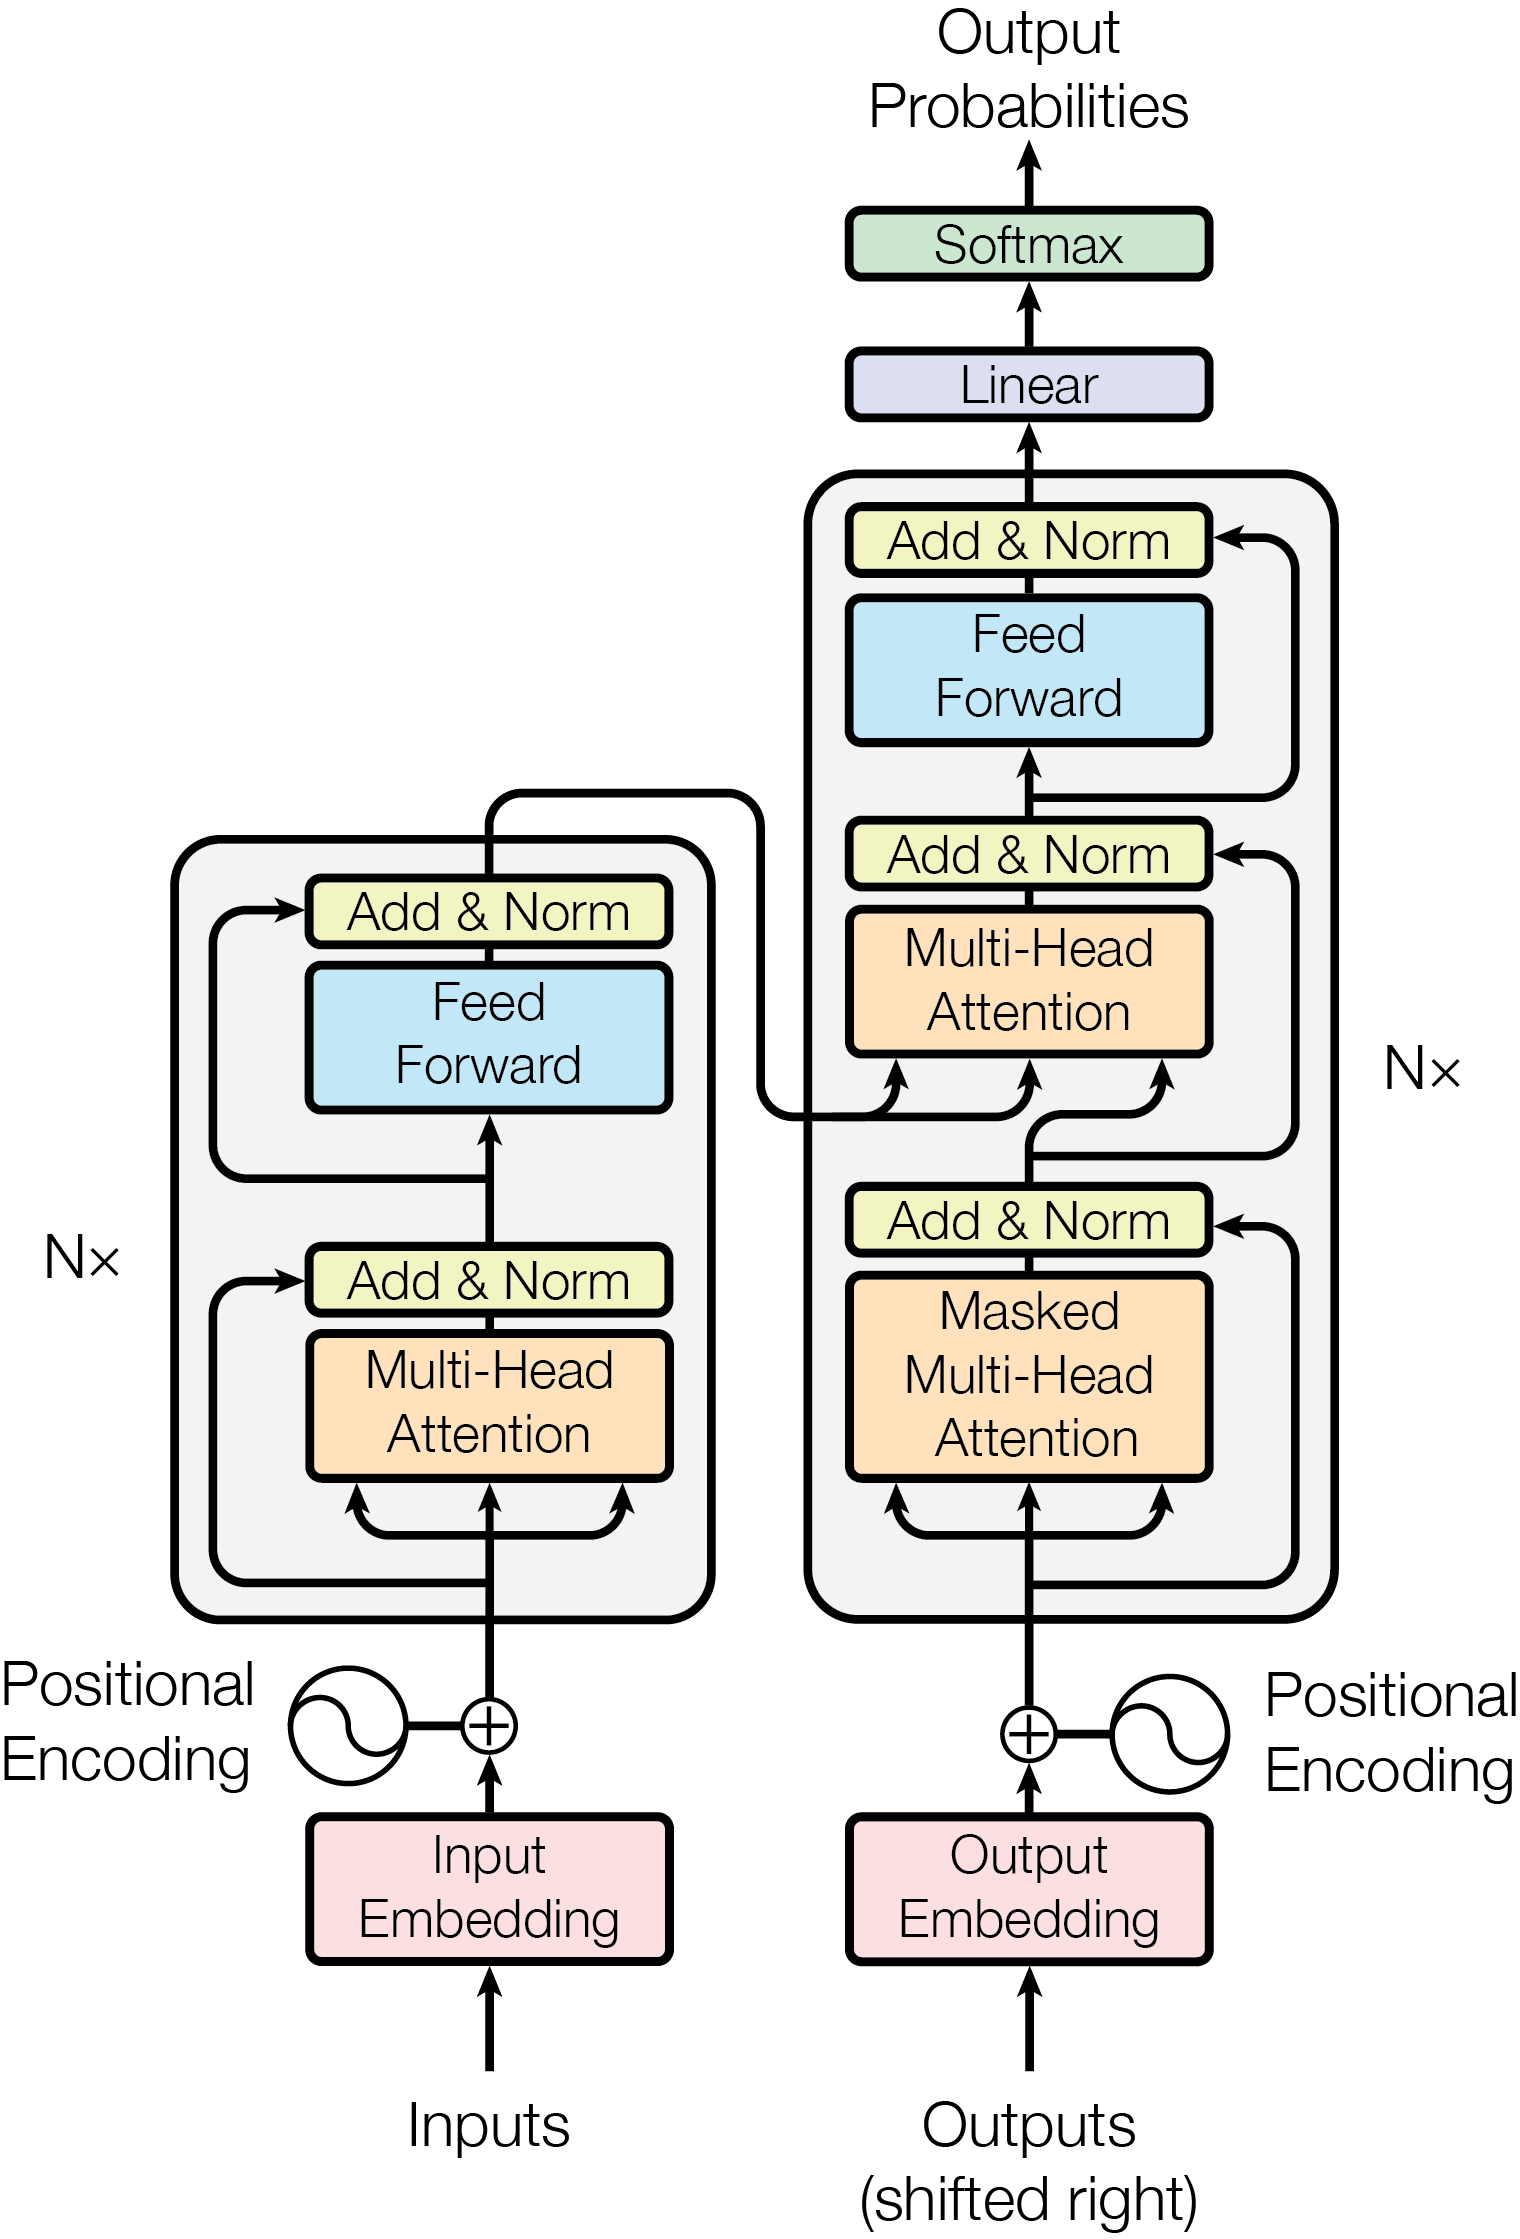
\includegraphics[scale=0.15]{Images & Logos/Transformers.png} 
	\label{figure:transformers}
\end{figure}
 

Gracias a la capacidad de paralelizacion y de conservar la relacion entre palabras distantes del texto que presentan los transformers, es posible entrenar un modelo del lenguaje con grandes volumenes de informacion para de esta manera, contar con una red con un gran poder predictivo. Es así como\cite{devlin2018bert}  desarrolla un modelo basado en Transformers capaz de aprender el contexto del lenguaje de una manera general y luego utilizar lo aprendido para distintas tareas de NLP denominado BERT (Bidirectional Transformers for Language Understanding). Para ello se utilizo una arquitectura en donde las capas de entrada son las representaciones vectoriales de las palabras (Embedings) y a partir de ahí, contiene múltiples capas de Transformers. Para su entrenamiento, esta arquitectura tuvo dos tareas simultaneas: se suministran dos oraciones consecutivas con palabras faltantes y las tareas son saber que palabra podría ser la faltante, ademas de identificar el orden de las oraciones. Esto le permite al modelo aprender del contexto del lenguaje a nivel de palabras usando las que vienen antes y después como fuente de información, así como del contexto de las oraciones al identificar su orden. Para ello se utilizo toda la wikipedia. Este modelo pre entrenado es luego capaz de utilizar esta representación contextual del lenguaje para realizar distintas tareas de NLP tales como análisis de sentimiento, al agregar una capa final a la red que produzca un posible resultado y al comparar este con su respectivo valor esperado realizar un entrenamiento. El esquema de esta arquitectura se puede apreciar en \ref{figure:BERT} \cite{devlin2018bert}.

\begin{figure}[h]
	\caption{Arquitectura de BERT}
	\centering
	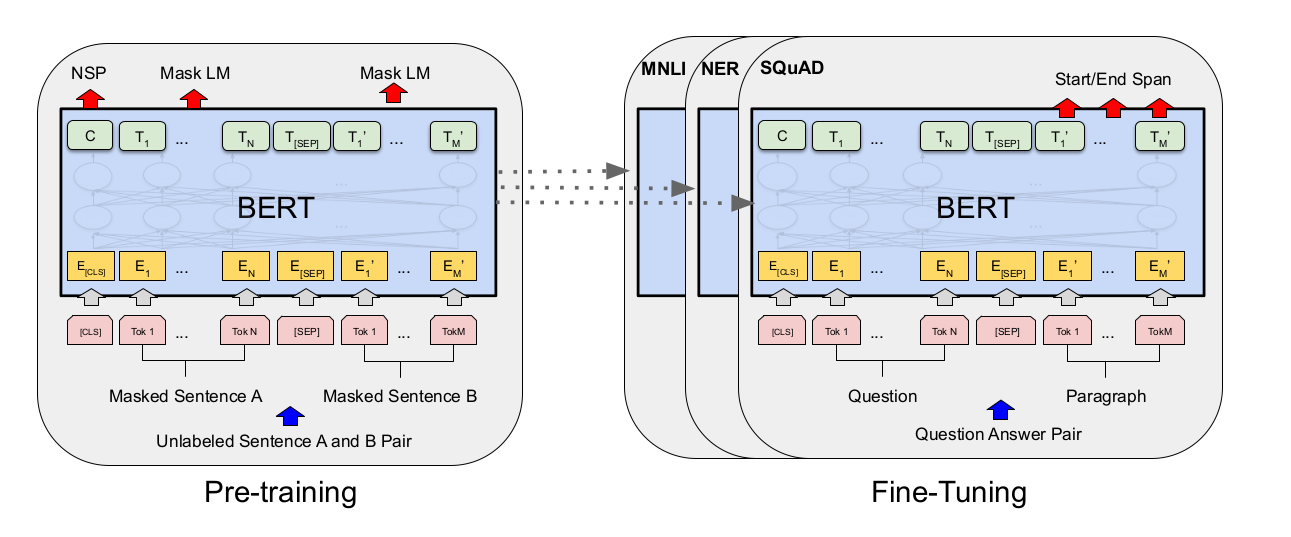
\includegraphics[scale=0.35]{Images & Logos/BERT.png} 
	\label{figure:BERT}
\end{figure}



\subsection{Detección de sentimientos y emociones en español}

Las técnicas y desarrollos relativos al análisis de emociones y sentimientos, provienen inicialmente del ingles. Una vez se cuenta con un marco metodológico en funcionamiento para este idioma, se desarrollan esfuerzos para su aplicación en otros, como el español. En este contexto, debido a la necesidad de contar con términos en español que puedan ser relacionados a determinadas emociones para propósitos de la detección automática, \cite{sidorov2012empirical} provee un léxico con tal propósito, que obtienen a través de la traducción de léxicos semejantes en ingles, que son luego evaluados por comentadores individuales, para filtrar aquellas palabras que presenten poca asociación con las emociones, así como dar un porcentaje de asociación del termino a la emoción, dependiendo de cuantos comentadores estuvieron de acuerdo en dicha asosiacion. En un esfuerzo similar por contar con texto en español, asi como para arabe, etiquetado para el dominio de detección emocional,\cite{mohammad2018semeval} se identifica términos claves en ingles asociados a las distintas emociones básicas. Estos términos fueron luego traducidos, verificados por hablantes nativos y expandidos utilizando sus sinónimos, para luego ser utilizados como parte de la query a la API de twitter y a partir de ahí, se procede a un etiquetado manual de los tweets a través de una plataforma de crowdsourcing. Esfuerzos similares para llevar a cabo el etiquetado manual de los tweets fueron llevados a cabo por \cite{sidorov2016construccion} en donde los terminos emocionales fueron usados como hashtags a la hora de hacer los llamados a la api, para tweets de distintos paises y luego fueron verificados a mano. Por otro lado, \cite{plaza2020emoevent} creo asi mismo un set de datos de tweets con contenido emocional.

Estos esfuerzos previos son aprovechados por \cite{plaza2020improved} donde se identifica que existe poca literatura al rededor de la clasificación de emociones en texto en español. Para ello, se plantea la evaluación de distintos modelos de aprendizaje supervisado usando el corpus de tweets en español con categorías emocionales provenientes de \cite{mohammad2018semeval}. A partir de ahí, se  procede a generar  representaciones vectoriales de los tweets. Se evalúan luego estos modelos de para tener un desempeño de base y luego se añade una variable que indique la presencia de algunos términos claves asociados con las emociones básicas, proveniente del trabajo realizado por \cite{sidorov2012empirical}. Esto mejoro considerablemente el desempeño del modelo. Un esfuerzo similar realizo \cite{gil2013combining} quien lleva a cabo una clasificación con supervisado distante de las emociones. Para dicho propósito recurre al empleo de términos relacionados con algunas de las emociones básicas como hashtags a la hora de realizar la query a la API y se construye un dataset en donde los tweets que contengan dichos hashtags son pertenecientes a determinada emoción. A partir de ahí se entrenan distintos algoritmos de aprendizaje supervisado.

Si bien estos esfuerzos sirvieron para sentar las bases del desarrollo del area de detección de emociones en español, así como en ingles, carecen de métodos que les permitan tener en cuenta la informacion contextual del texto. En ese sentido, con el desarrollo de las técnicas de NLP basadas en redes neuronales en ingles, surgieron así mismo esfuerzos para aplicar dichas técnicas en el dominio del texto en español. Es así como en \cite{canete2020spanish} se destaca la importancia de los modelos pre entrenados basados en Transformers por su superior desempeño en tareas de NLP ademas de su practicidad de uso. Sin embargo, resaltan que no existía hasta la fecha un modelo de este tipo entrenado específicamente para español, ademas del BERT para múltiples lenguajes. Por ello, se proponen entrenar dicho modelo usando ademas de la Wikipedia en español, texto de publicaciones de las naciones unidas, gobiernos y charlas TED. El resultado fue un modelo que supera al BERT en múltiples idiomas para el español en casi todas las tareas evaluadas.Un es fuerzo similar llevo a cabo \cite{gonzalez2021twilbert} donde se resaltan las ventajas de la arquitectura de BERT, sin embargo se pone de manifiesto que el idioma español en general y el dominio de twitter en particular, poseen características propias que al ser tenidas en cuenta, podrían mejorar el desempeño para esta tarea en especifico con respecto al modelo de múltiples lenguaje de BERT. Para ellos, se recurre a un corpus de 41 millones de tweets en español con el que se entrena un modelo con la arquitectura de BERT al que denominan TwilBert, obteniendo resultados mejores que BERT para algunas tareas de NLP







